\documentclass[11pt]{article}
\usepackage[margin=1in]{geometry}
\usepackage{enumitem}
\usepackage{hyperref}
\usepackage{graphicx}
\usepackage{array}
\usepackage{multicol}
\usepackage{longtable}
\usepackage{titlesec}
\usepackage{amsmath} 
\usepackage{float} % Required for [H] placement

\begin{document}

\begin{center}
    \large \textbf{Sri Sivasubramaniya Nadar College of Engineering, Chennai} \\
    (An autonomous Institution affiliated to Anna University) \\
    \vspace{0.3cm}
\end{center}

\begin{table}[h]
\renewcommand{\arraystretch}{1.4}
\resizebox{\textwidth}{!}{%
\begin{tabular}{|l|l|l|l|}
\hline
Degree \& Branch & B.E. Computer Science \& Engineering & Semester & VI \\ \hline
Subject Code \& Name & \multicolumn{3}{l|}{UCS2612 – Machine Learning Algorithms Laboratory} \\ \hline
Academic Year & 2025–2026 (Even) & Batch & 2023–2027 \\ \hline
Name & Kushaal Shyam Potta & Register No. & 3122235001071 \\ \hline
Due Date & \multicolumn{3}{l|}{02.01.2026} \\ \hline
\end{tabular}}
\end{table}

\begin{center}
 \textbf{Experiment 1: Working with Python packages -- Numpy, Scipy, Scikit-Learn, Matplotlib}
\end{center}

\noindent \textbf{Aim:} \\
To investigate and utilize Python libraries such as NumPy, Scikit-learn, and Matplotlib on public repository datasets to determine machine learning objectives, feature selection strategies, and appropriate predictive algorithms.
\vspace{0.5cm}
\noindent
\textbf{Libraries used:}
\begin{itemize}[noitemsep]
    \item NumPy (imported as \texttt{np})
    \item Pandas (imported as \texttt{pd})
    \item Matplotlib.pyplot (imported as \texttt{plt})
    \item Seaborn (imported as \texttt{sns})
    \item OpenCV (\texttt{cv2})
    \item StandardScaler (from sklearn.preprocessing)
    \item Math (Standard Library)
    
\end{itemize}
\vspace{0.5cm}
\noindent
\textbf{Mathematical and Theoretical description of the objectives performed:}
\begin{itemize}
    \item \textbf{Purpose:} Conduct Exploratory Data Analysis (EDA) to investigate data characteristics, analyze distribution patterns, detect outliers, assess class balance, and distinguish dependencies between features.
     
    \item \textbf{Descriptive Statistics}
    \begin{itemize}
        \item Arithmetic mean calculated via: $\mu = \frac{1}{n} \sum x_i$
        \item Sample variance used to quantify data spread: $s^2 = \frac{1}{n-1} \sum (x_i - \mu)^2$
        \item Quantile statistics (Median, $Q1$, $Q3$) employed to evaluate dispersion and generate boxplots.
    \end{itemize}
     
    \item \textbf{Distribution Analysis Using Histograms}
    \begin{itemize}
        \item Approximation of empirical distributions through frequency binning to illustrate data shape and central tendencies.
        \item Application of Kernel Density Estimation (KDE) to provide a continuous estimation of the probability density:
        \[
        \hat{f}(x) = \frac{1}{nh} \sum_{i=1}^{n} K\left(\frac{x - x_i}{h}\right)
        \]
        where $K$ represents the kernel function and $h$ denotes the smoothing bandwidth.
    \end{itemize}
     
    \item \textbf{Boxplot Visualization}
    \begin{itemize}
        \item Representation of the median and quartiles ($Q1$, $Q3$), defining the interquartile range as $IQR = Q3 - Q1$.
        \item Whiskers delineate data within the boundary $[Q1 - 1.5 \cdot IQR, \ Q3 + 1.5 \cdot IQR]$; values residing outside this range are identified as statistical outliers.
    \end{itemize}
     
    \item \textbf{Feature Relationship Plots}
    \begin{itemize}
        \item Scatter plot matrices utilized for detecting trends, class separability, and non-linear correlations.
        \item Diagonal plots show individual feature distributions using histograms or KDEs.
    \end{itemize}
     
    \item \textbf{Correlation Visualization}
    \begin{itemize}
        \item Quantification of linear relationships between variables using the Pearson correlation coefficient:
        \[
        r_{XY} = \frac{\text{cov}(X,Y)}{\sigma_X \sigma_Y}
        \]
        \[
        \text{cov}(X,Y) = \frac{1}{n-1} \sum (X_i - \bar{X})(Y_i - \bar{Y})
        \]
        \item Coefficient values range from $[-1, 1]$, indicating both the strength and orientation of linear association.
    \end{itemize}
     
    \item \textbf{Categorical Data Visualization}
    \begin{itemize}
        \item Frequency-based bar charts used to analyze category counts and investigate potential class imbalances.
    \end{itemize}
    \item \textbf{Image Data Exploration}
    \begin{itemize}
        \item Analysis of image resolutions (height and width) via histograms or KDEs to ensure consistency for model input.
        \item Display of sample images to qualitatively evaluate visual data properties.
    \end{itemize}
     
    \item \textbf{Handling Missing Data}
    \begin{itemize}
        \item Feature-wise audit of null values to determine appropriate mitigation strategies, such as data imputation or pruning.
    \end{itemize}
    \item \textbf{Analytical Objectives}
    \begin{itemize}
        \item Identification of skewed data, multimodality, anomalous entries, collinear features, and class skews to facilitate effective preprocessing and model optimization.
    \end{itemize}
\end{itemize}


\vspace{1.5 cm}
\noindent
\textbf{Results and Discussions:}
\subsection{Loan Amount Prediction}

\begin{figure}[H]
    \centering
    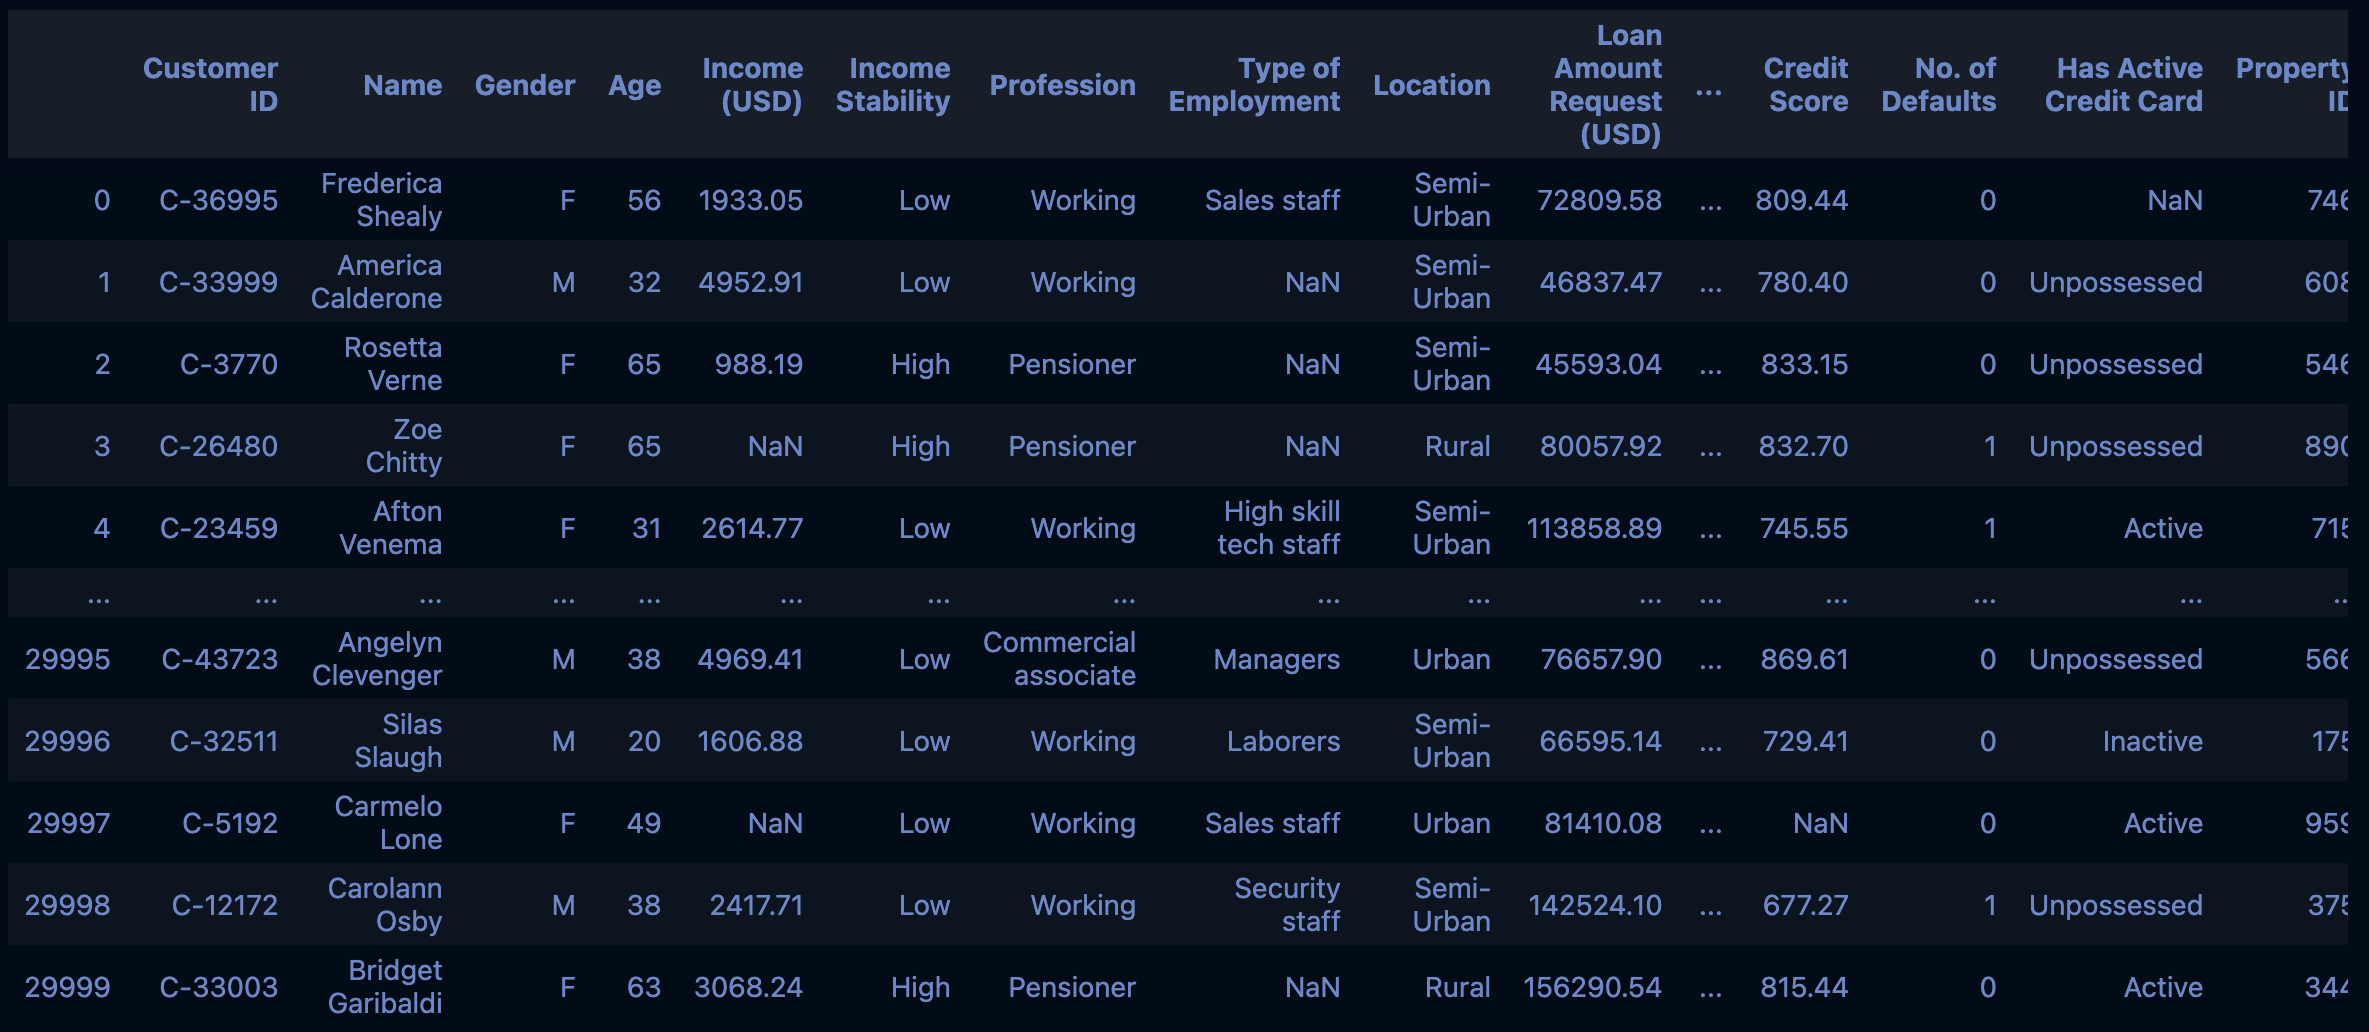
\includegraphics[width=0.75\linewidth]{loan_columns.png}
    \caption{Dataset Columns}
\end{figure}

\begin{figure}[H]
    \centering
    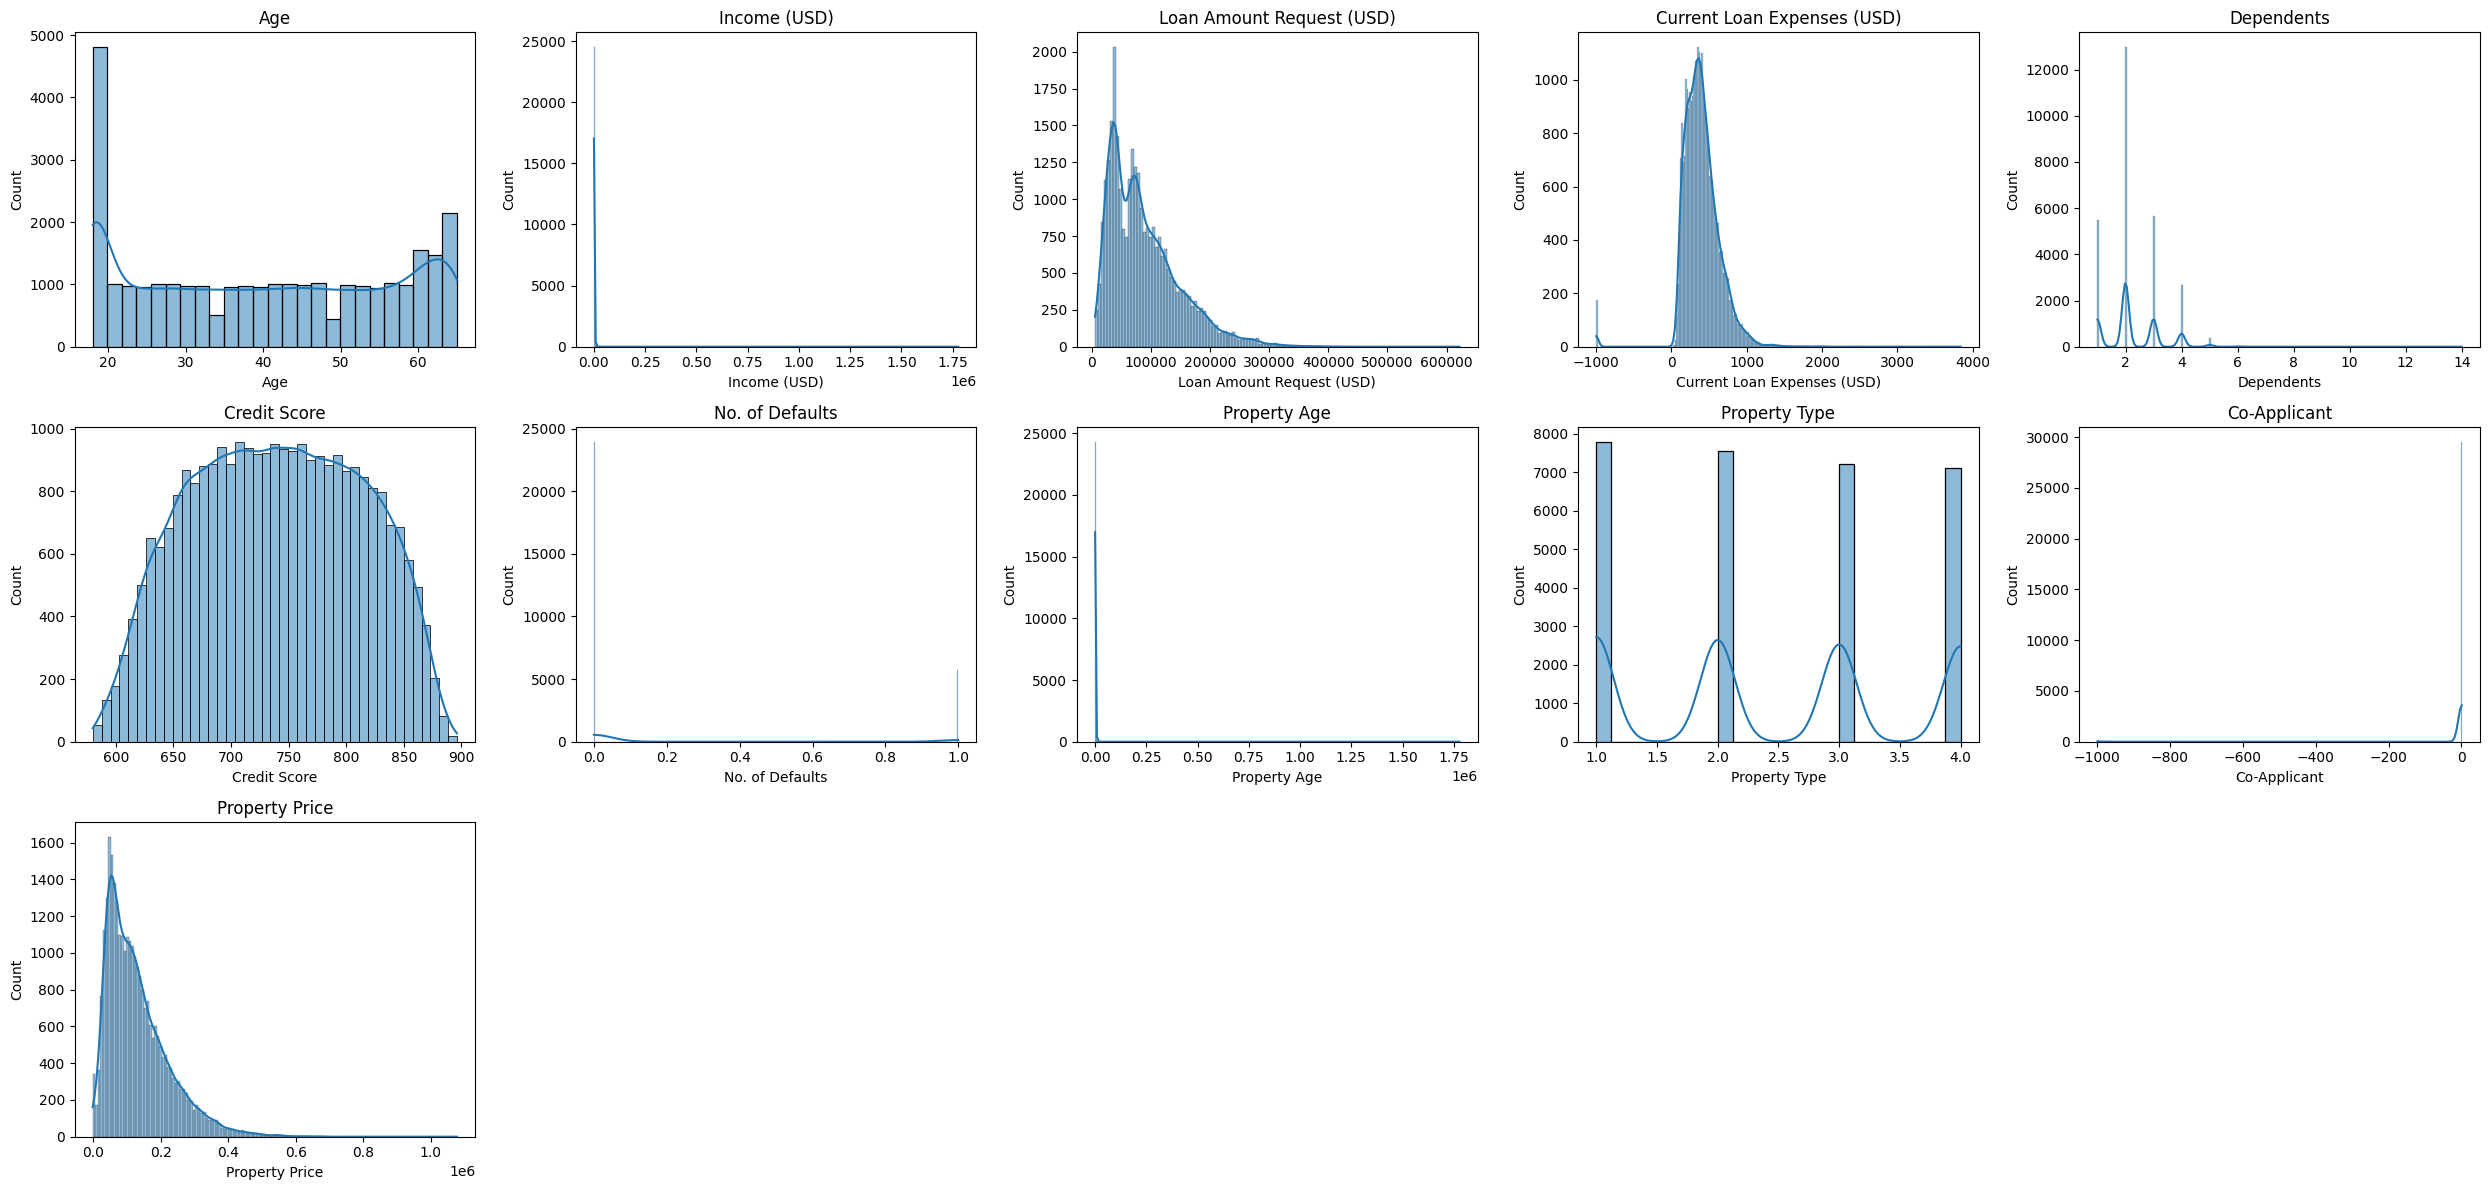
\includegraphics[width=\linewidth]{loan_distribution.png}
    \caption{Loan Amount Distribution (Histogram Plot)}
\end{figure}

\begin{figure}[H]
    \centering
    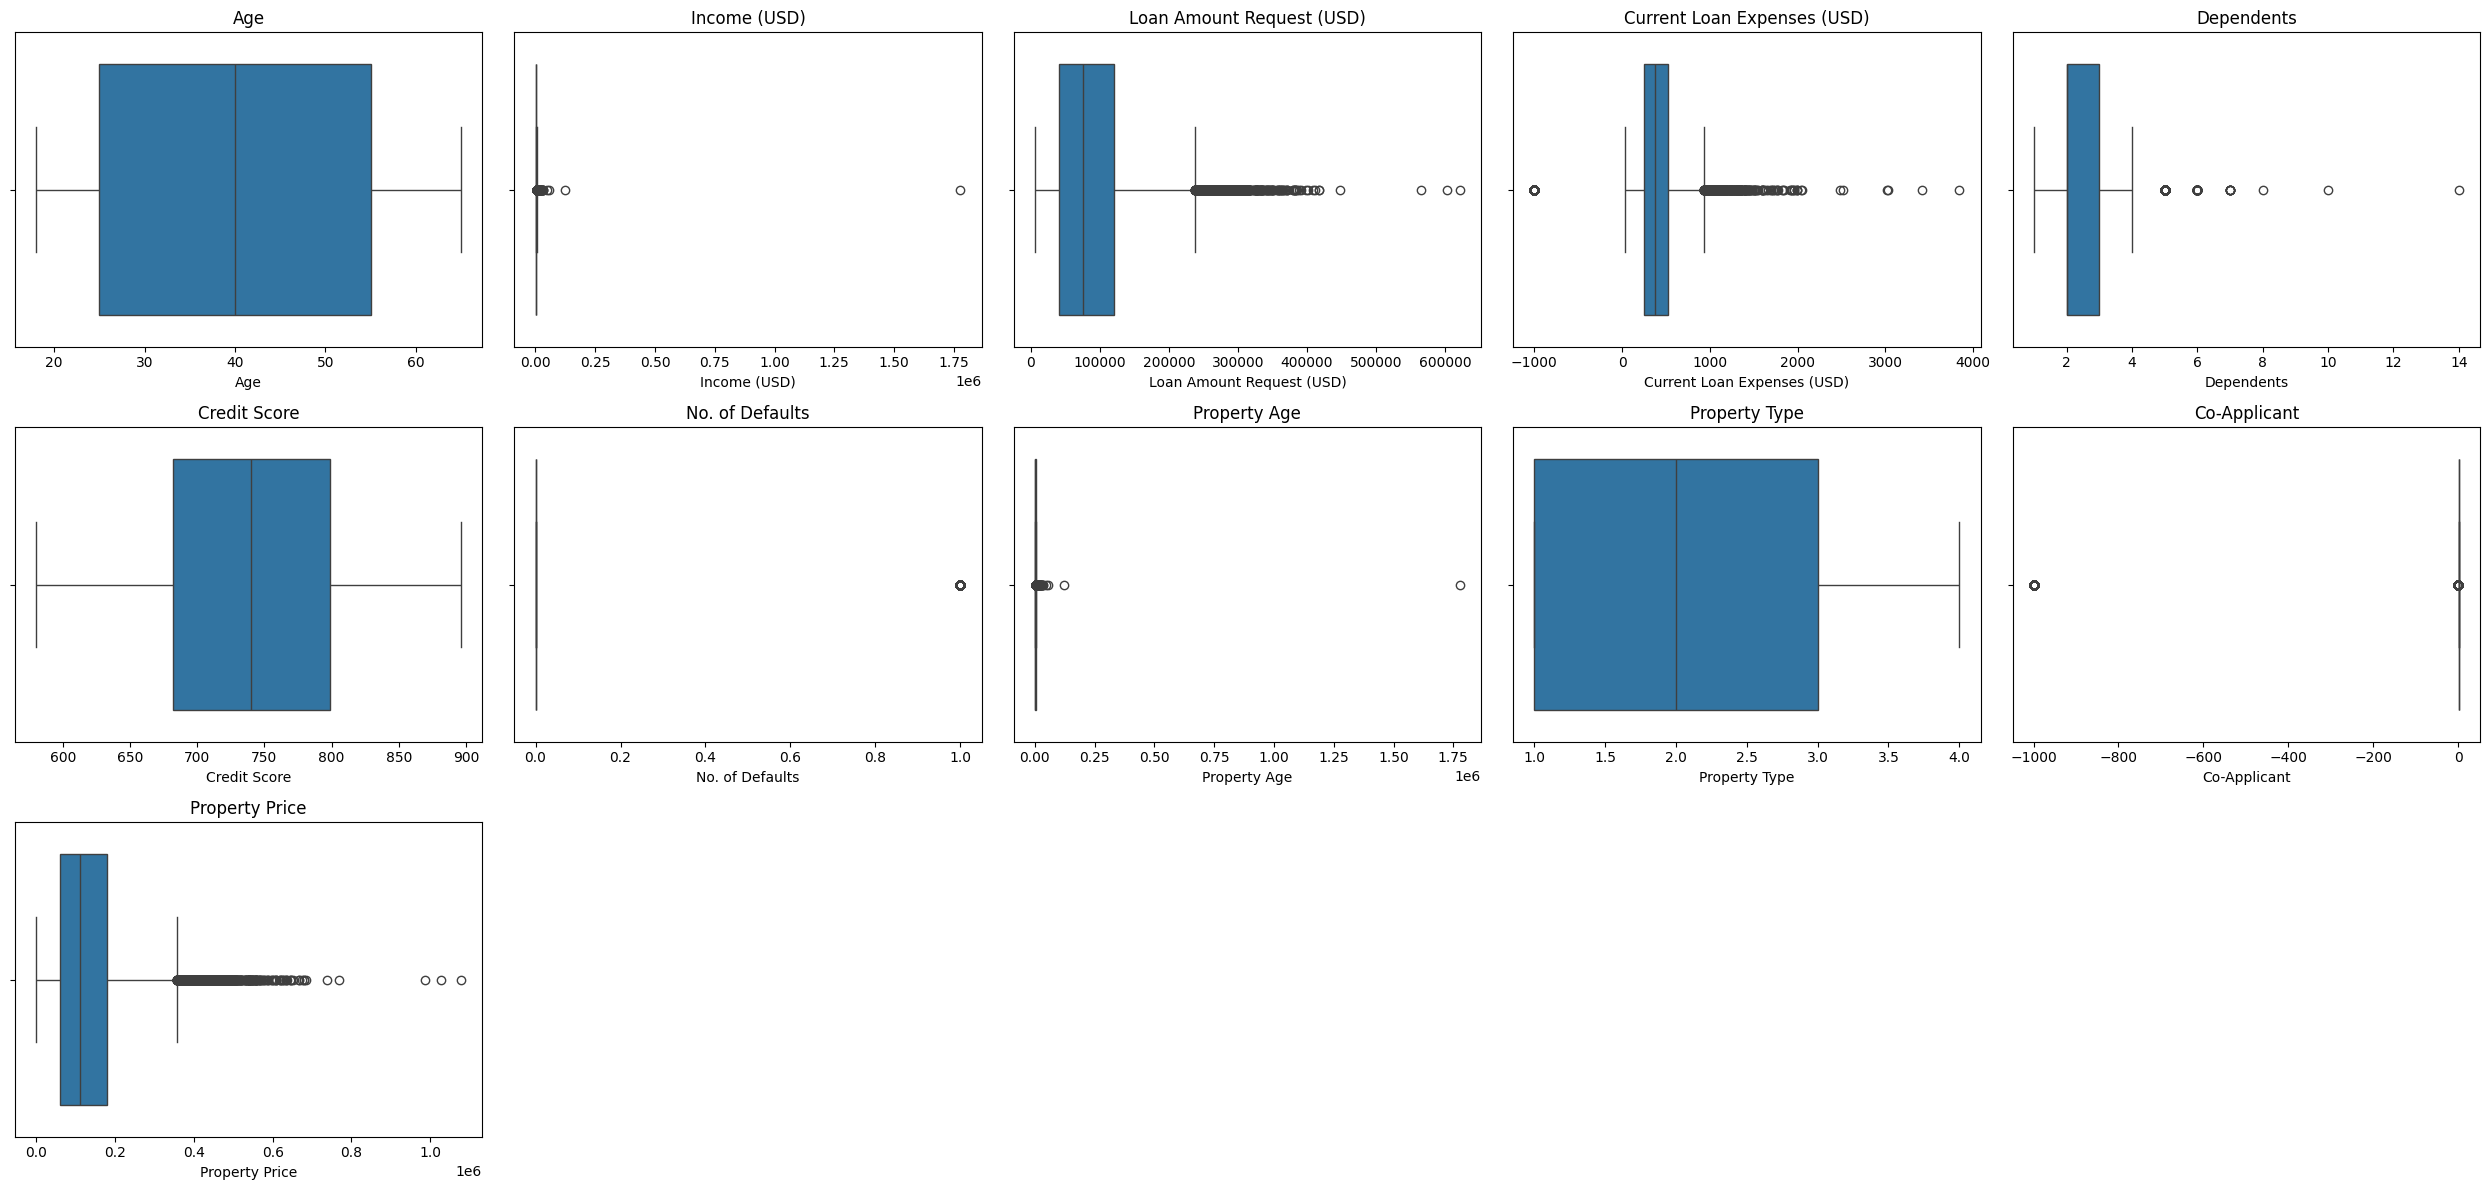
\includegraphics[width=\linewidth]{loan_boxplot.png}
    \caption{Boxplot Distribution}
\end{figure}

\begin{figure}[H]
    \centering
    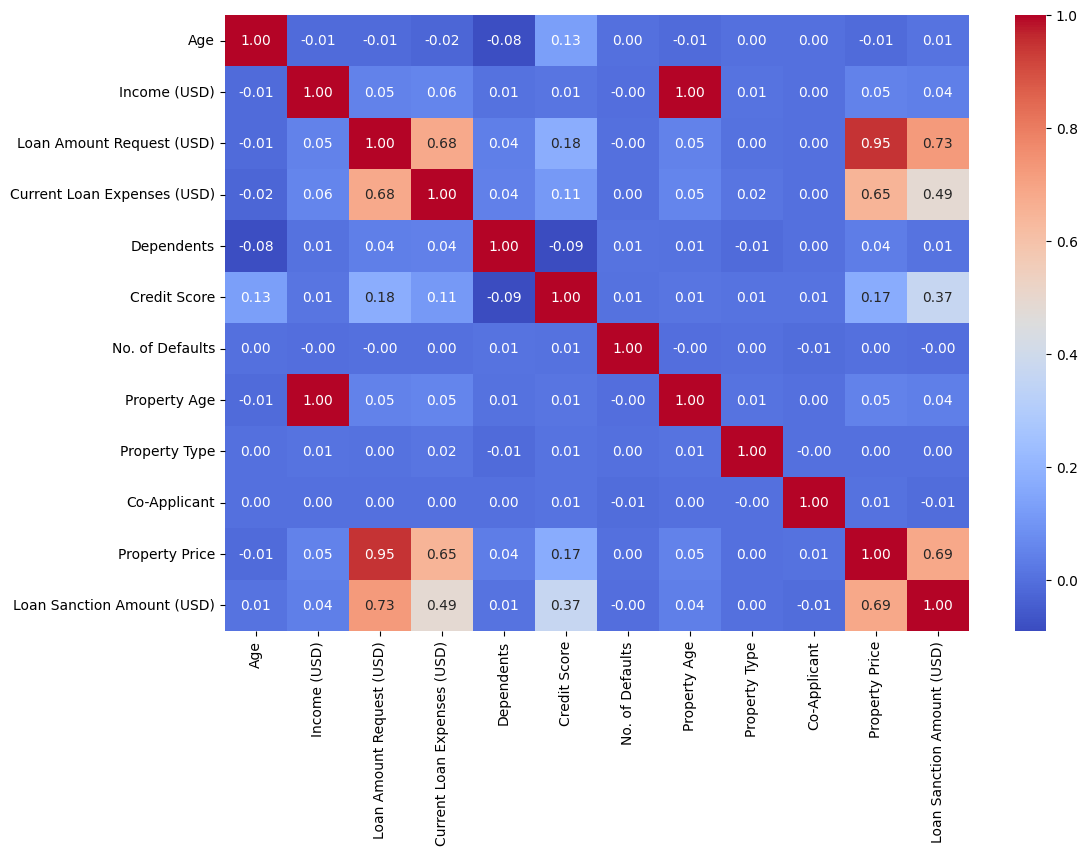
\includegraphics[width=0.75\linewidth]{loan_correlation.png}
    \caption{Correlation Matrix}
\end{figure}

\subsection{Handwritten Character Recognition (MNIST)}

\begin{figure}[H]
    \centering
    
\includegraphics[width=0.75\linewidth]{sample_images.png}
    \caption{Sample Images}
\end{figure}


\begin{figure}[H]
    \centering
    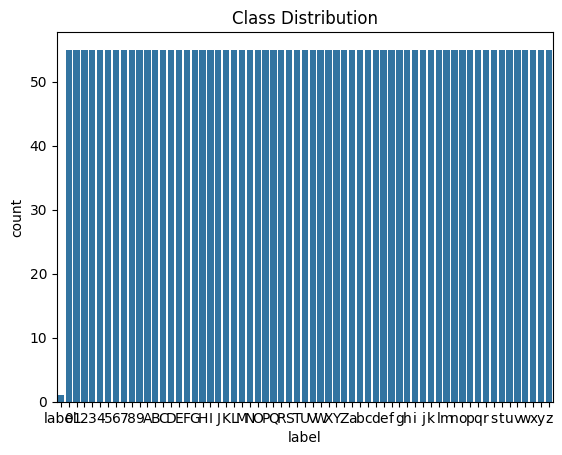
\includegraphics[width=\linewidth]{minst_distribution.png}
    \caption{Digit Distribution}
\end{figure}

\begin{figure}[H]
    \centering
    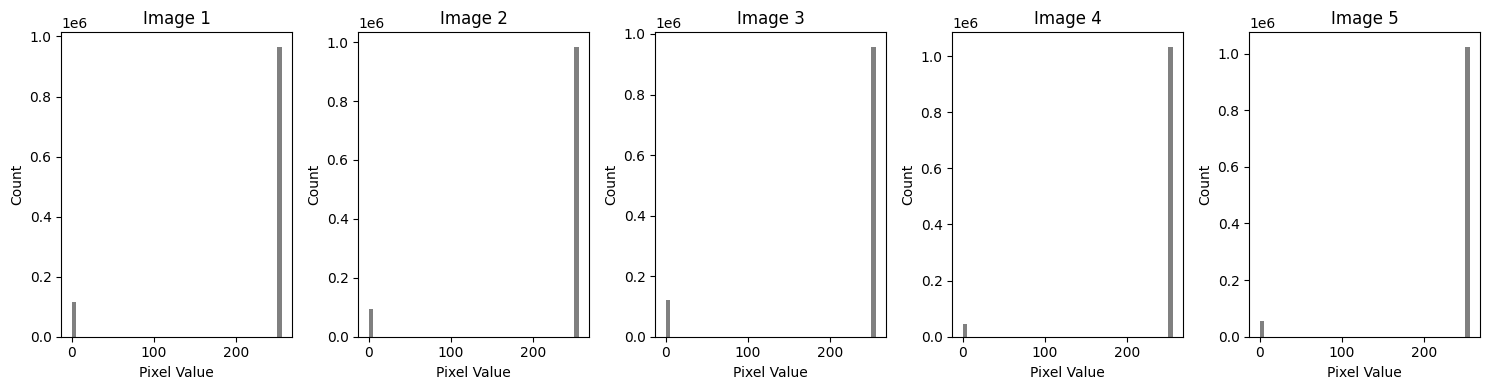
\includegraphics[width=\linewidth]{mnist_pixel_intensity.png}
    \caption{Pixel Intensity Analysis}
\end{figure}

\begin{figure}[H]
    \centering
    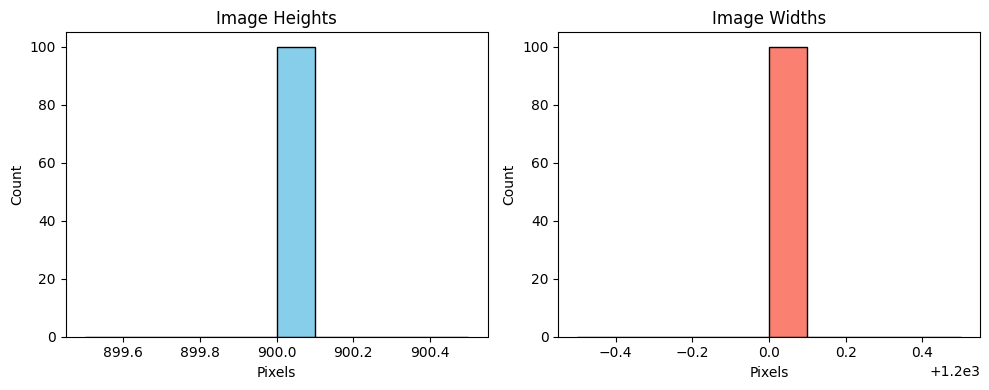
\includegraphics[width=0.75\linewidth]{mnist_hw.png}

    \caption{Height Weight Distribution}
\end{figure}

\subsection{Classification of Email Spam}
\begin{figure}[H]
    \centering
    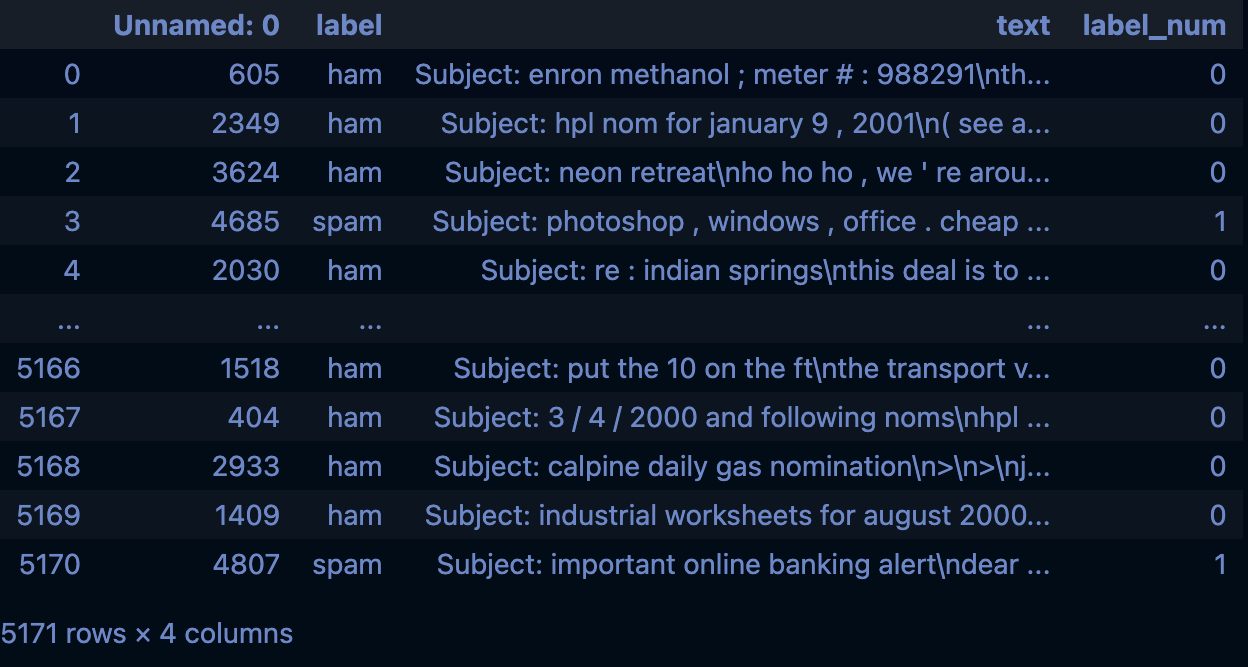
\includegraphics[width=0.75\linewidth]{spam_ham_columns.png}
    \caption{Dataset Columns}
\end{figure}

\begin{figure}[H]
    \centering
    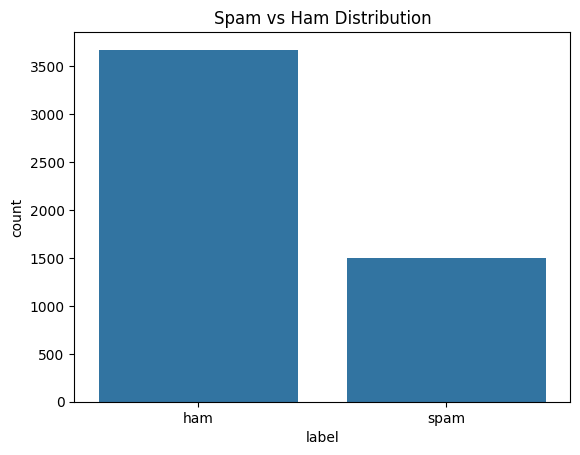
\includegraphics[width=0.75\linewidth]{spam_ham_features.png}
    \caption{Spam vs Ham Distribution}
\end{figure}

\begin{figure}[H]
    \centering
    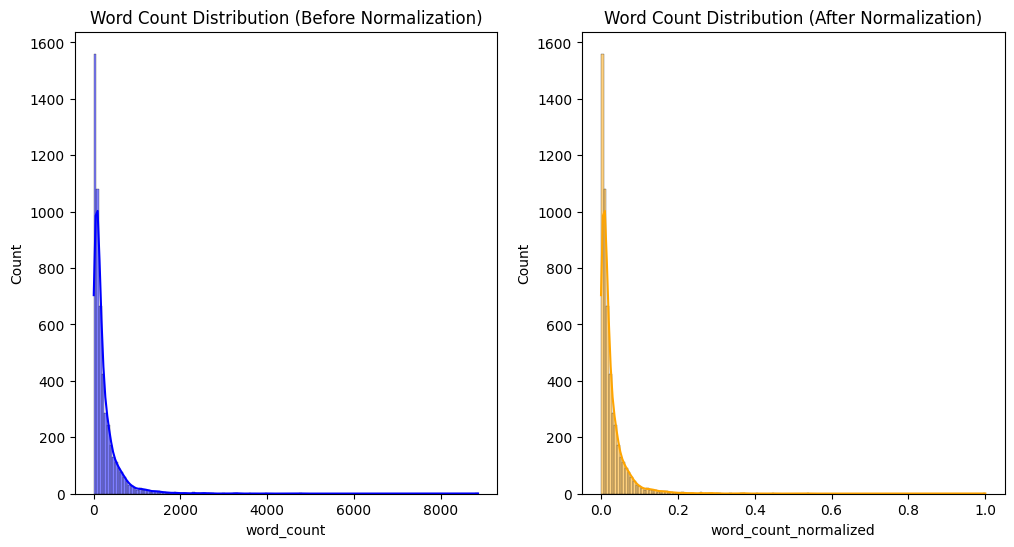
\includegraphics[width=\linewidth]{word_count_distirubtion.png}
    \caption{Word Count Distribution (Normalisation)}
\end{figure}

\begin{figure}[H]
    \centering
    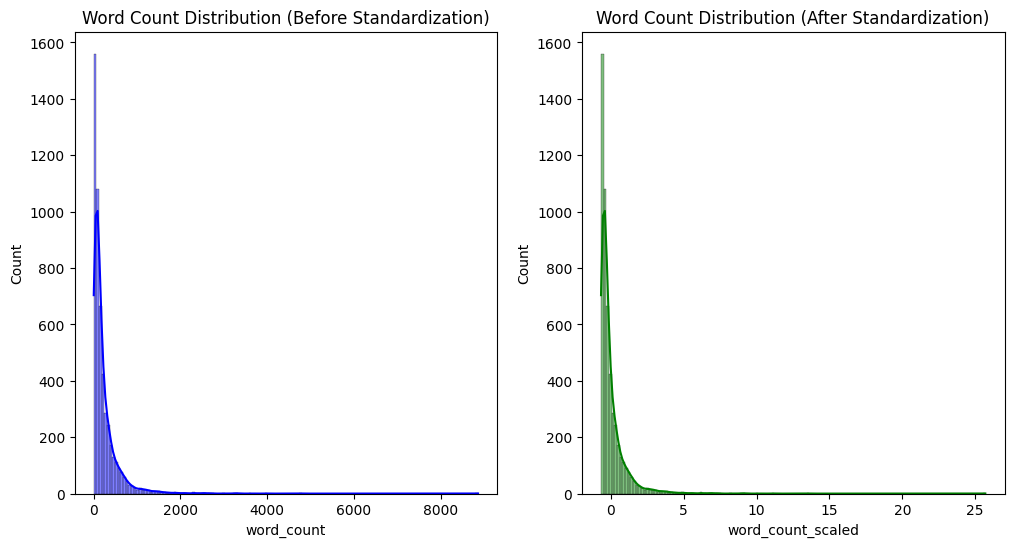
\includegraphics[width=\linewidth]{word_count_distirubtion_1.png}
    \caption{Word Count Distribution (Standardisation)}
\end{figure}

\begin{figure}[H]
    \centering
    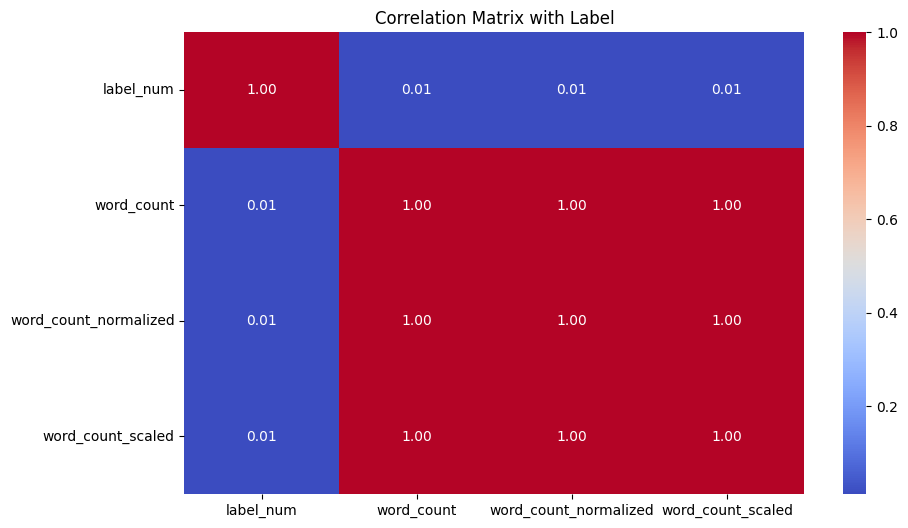
\includegraphics[width=0.75\linewidth]{spam_correlation.png}
    \caption{Correlation Matrix}
\end{figure}
\begin{figure}[H]
    \centering
    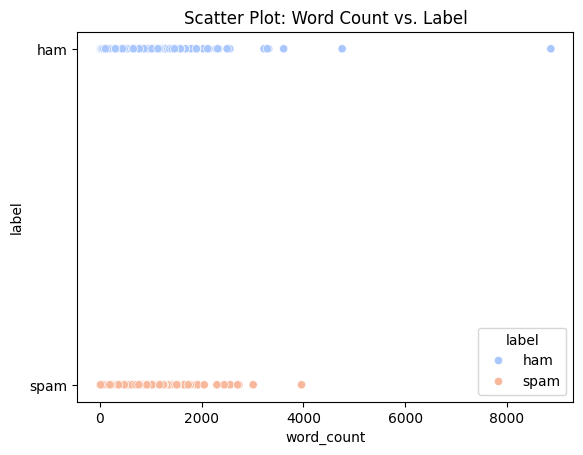
\includegraphics[width=0.75\linewidth]{word_scatterplot.png}
    \caption{Scatter Plot}
\end{figure}

\subsection{Predicting Diabetes}

\begin{figure}[H]
    \centering
    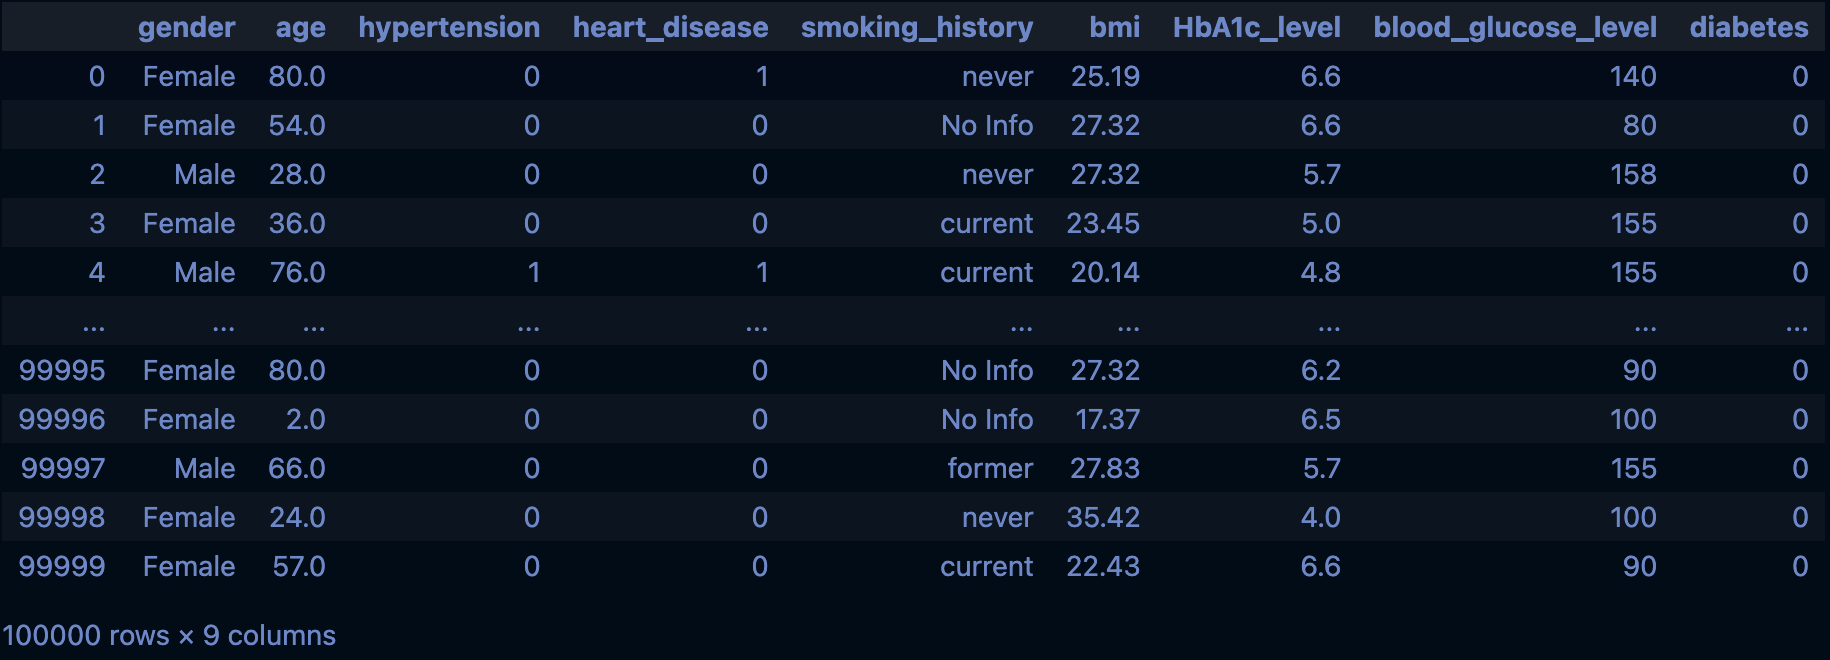
\includegraphics[width=0.75\linewidth]{diabetes_columns.png}
    \caption{Dataset Columns}
\end{figure}

\begin{figure}[H]
    \centering
    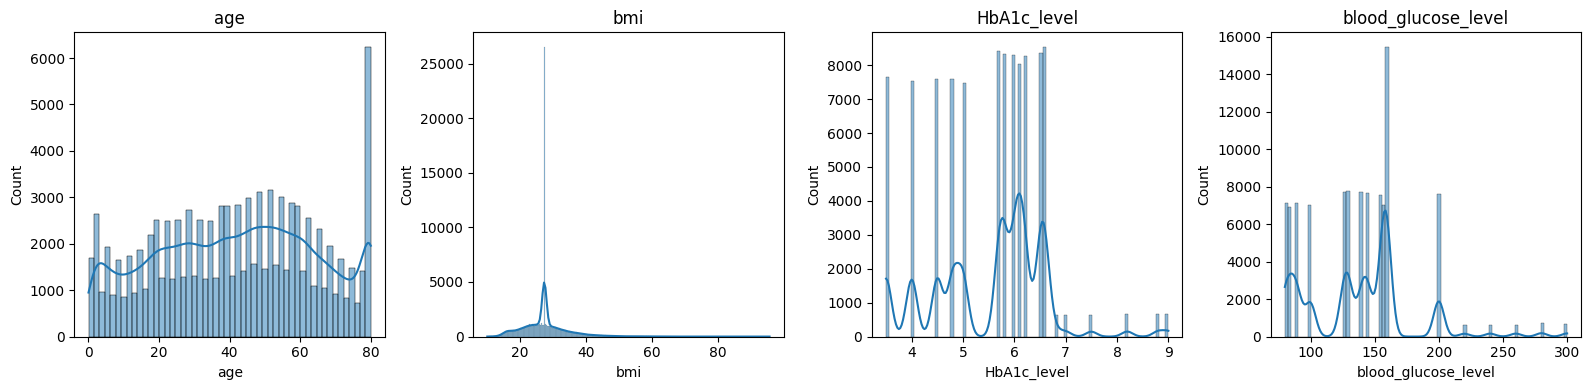
\includegraphics[width=\linewidth]{diabetes_distribution.png}
    \caption{Histogram Distribution}
\end{figure}

\begin{figure}[H]
    \centering
    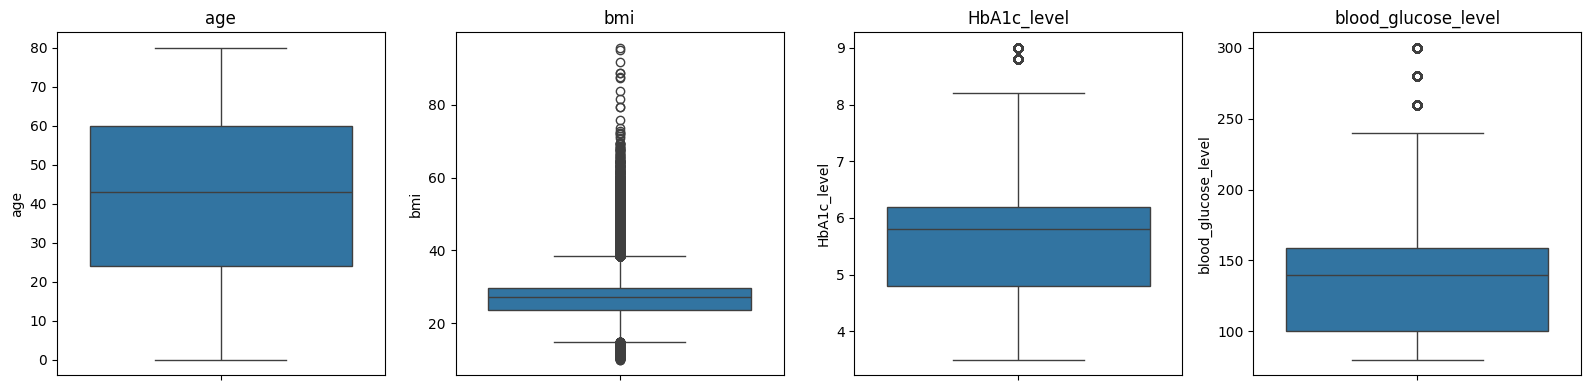
\includegraphics[width=\linewidth]{diabetes_boxplot.png}
    \caption{Boxplot distribution}
\end{figure}

\begin{figure}[H]
    \centering
    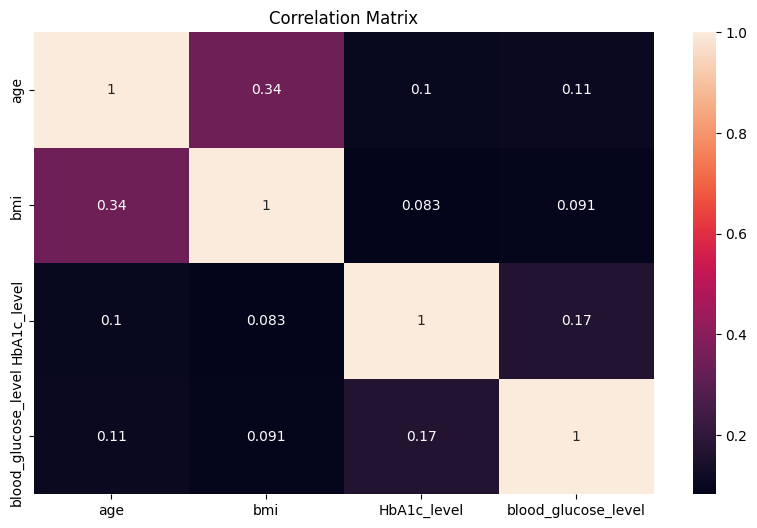
\includegraphics[width=0.75\linewidth]{diabetes_correlation.png}
    \caption{Correlation Matrix}
\end{figure}


\subsection{Iris Dataset}

\begin{figure}[H]
    \centering
    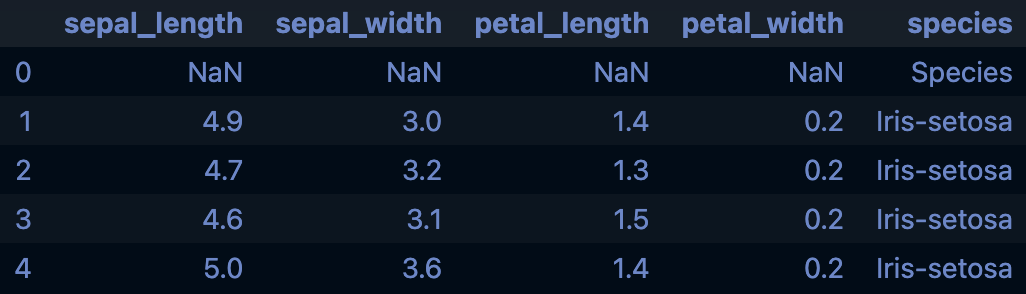
\includegraphics[width=0.75\linewidth]{iris_columns.png}
    \caption{Dataset Columns}
\end{figure}

\begin{figure}[H]
    \centering
    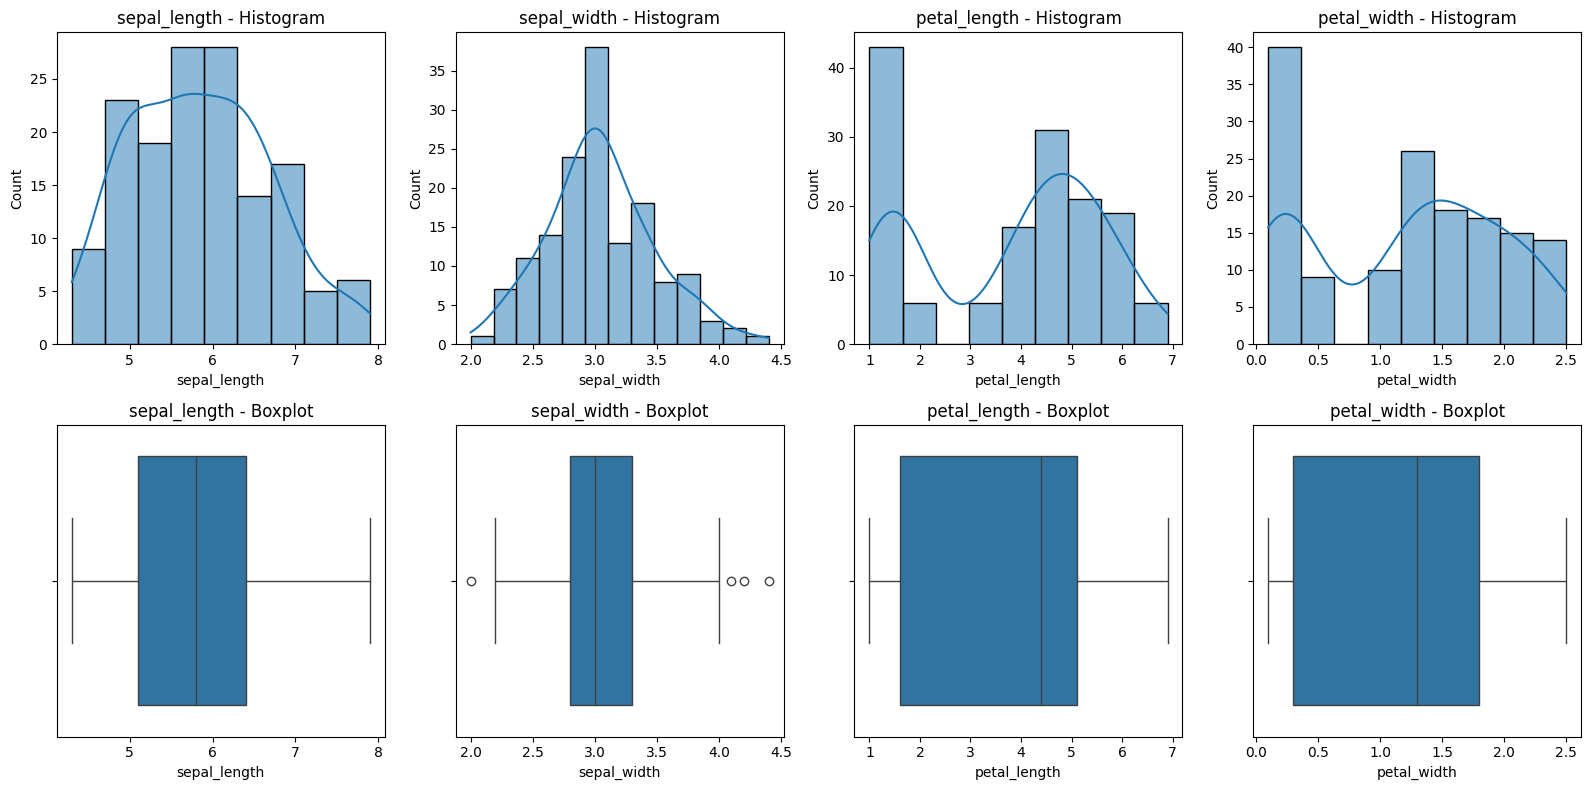
\includegraphics[width=\linewidth]{iris_hist_box.png}
    \caption{Histogram and Boxplot Distribution}
\end{figure}

\begin{figure}[H]
    \centering
    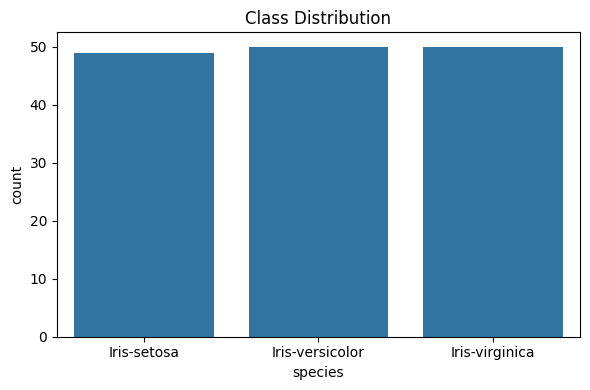
\includegraphics[width=\linewidth]{iris_class.png}
    \caption{Class Distribution}
\end{figure}

\begin{figure}[H]
    \centering
    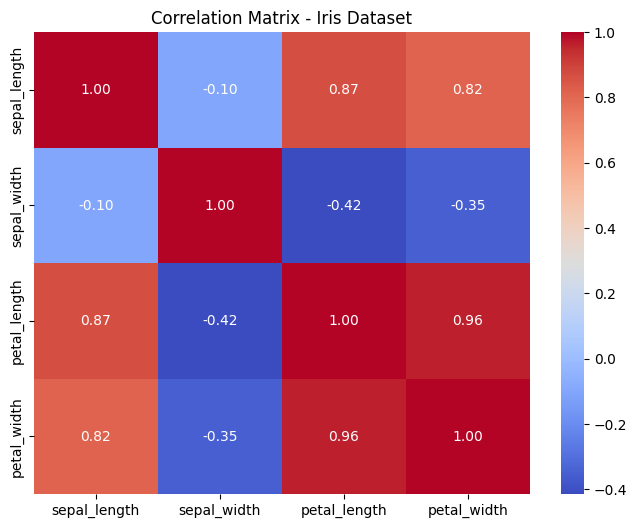
\includegraphics[width=0.75\linewidth]{iris_correlation.png}
    \caption{Correlation Matrix}
\end{figure}



\begin{table}[H] 
\centering
\vspace{0.5cm}
\renewcommand{\arraystretch}{1.5}
\begin{tabular}{|p{0.15\textwidth}|p{0.22\textwidth}|p{0.28\textwidth}|p{0.25\textwidth}|}
\hline
\textbf{Dataset} & \textbf{Type of ML Task} & \textbf{Feature Selection Technique} & \textbf{Suitable ML Algorithm} \\ \hline
Iris Dataset & Multi-class Classification & Correlation Matrix / ANOVA F-value & k-Nearest Neighbors (k-NN), Decision Trees \\ \hline
Loan Amount Prediction & Regression & Recursive Feature Elimination (RFE) / Pearson Correlation & Linear Regression, Random Forest Regressor \\ \hline
Predicting Diabetes & Binary Classification & Chi-Square Test / SelectKBest & Logistic Regression, Support Vector Machine (SVM) \\ \hline
Classification of Email Spam & Binary Classification (NLP) & Information Gain / Chi-Square (on word vectors) & Naive Bayes, SVM \\ \hline
Handwritten Character Recognition / MNIST & Multi-class Image Classification & Principal Component Analysis (PCA) & Convolutional Neural Networks (CNN), SVM \\ \hline
\end{tabular}
\end{table}
\vspace{0.5cm}
\noindent
\textbf{Learning Practices:}
\begin{itemize}
    \item Investigate dataset structure: Comprehend the organization by evaluating dimensions, variable types, and null value occurrences.
\item Study data characteristics: Build proficiency in pattern visualization through histograms, boxplots, and correlation heatmaps.
\item Evaluate class distribution: Examine label equilibrium and its impact on predictive performance and model reliability.
\item Examine variable dependencies: Study interdependencies between attributes using pairwise visualizations and correlation metrics.
\end{itemize}

\vspace{0.5cm}

\end{document}